%%%%%%%%%%%%%%%%%%%%%%%%%%%%%%%%%%%%%%%%%%%%%%%%%%%%%%%%%%%%%%%%%%%%%%
% How to use writeLaTeX: 
%
% You edit the source code here on the left, and the preview on the
% right shows you the result within a few seconds.
%
% Bookmark this page and share the URL with your co-authors. They can
% edit at the same time!
%
% You can upload figures, bibliographies, custom classes and
% styles using the files menu.
%
%%%%%%%%%%%%%%%%%%%%%%%%%%%%%%%%%%%%%%%%%%%%%%%%%%%%%%%%%%%%%%%%%%%%%%

\documentclass[12pt]{article}

\usepackage{sbc-template}

\usepackage{graphicx,url}

%\usepackage[brazil]{babel}   
\usepackage[utf8]{inputenc}  

     
\sloppy

\title{Banco de dados em memória secundária\\ Clubes de futebol - AEDs III}

\author{Bruno R. Faria\inst{1}, Breno Lopes\inst{2}}


\address{Ciências da Computação - Pontifícia Universidade Católica de Minas Gerais}

\begin{document} 

\maketitle
     
\begin{resumo} 
  Este documento descreve como foi possível a montagem de um sistema em terminal, simulando o acesso a um banco de dados. Capaz de adicionar times e fazer operações CRUDs no mesmo. O intuito do trabalho foi o entendimento de memória secundária, arquivos de dados estruturados e arquivo sequencial e indexado. Além de implementar uma lista invertida, uma busca binária para substituir as buscas sequenciais e uma ordenação interna no arquivo de índices, para sempre manter a ordenação. O trabalho foi realizado em linguagem de programação Java com controle de versões pela plataforma GitHub. O projeto é composto por três classes CRUD.java, Main.java e Clubes.java, os quais serão descritos no documento.
\end{resumo}

%%%%%%%%%%%%%%%%%%%%%%%%%%%%%%%%%%%%%%%%%%%%%%%%%%%%%%%%%%%%%%%%%%%%%%

\section{Introdução}

Para o início do desenvolvimento do projeto foi feita a seguinte pergunta: É necessário que se tenha a criação dos arquivos utilizados no programa ao iniciar, caso o arquivo não exista? A resposta para a pergunta foi simples, sim por conta de erros que poderiam ocorrer. Para iniciar o programa foi feito dentro do construtores das classes utilizadas uma código capaz de criar os arquivos necessário para todo o programa funcionar, o qual serviria de banco de dados para todos os dados inseridos pelo usuário, o da lista invertida serviria para armazenar a lista e o da ordenação externa e arquivo de indices para fazer a ordenação em memória secundária e para aramzenar os dados do arquivo original, respectivamente. Com os arquivos criados, poderia dar inicio ao projeto com maior tranquilidade, tanto para os programadores quanto para o próprio usuário.

%%%%%%%%%%%%%%%%%%%%%%%%%%%%%%%%%%%%%%%%%%%%%%%%%%%%%%%%%%%%%%%%%%%%%%

\section{Desenvolvimento} \label{sec:firstpage}

Para iniciar o desenvolvimento, após a criação do construtor da classe CRUD no qual iria inicializar o arquivo e a inserção do ID = -1 no inico do arquivo, deveria ser feito a classe Clube.java, na qual seria importante criar todos os atributos de um clubes de futebol e as funções que teriam interações com o clube. 

\begin{figure}[ht]
\centering
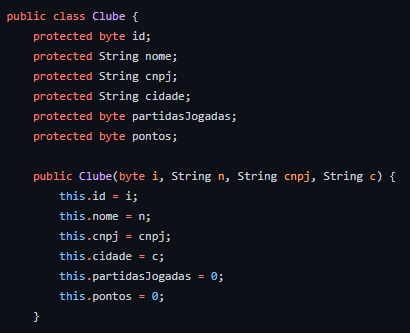
\includegraphics[width=.5\textwidth]{clubes.jpeg}
\caption{Construtor e atribuitos dos clubes}
\label{fig:exampleFig1}
\end{figure}

Os tipos de dados utilizados nas variáveis foram escolhidos de uma forma e não utilizar uma quantidade de Bits maior do que a necessária, um exemplo é o atributo ID onde foi colocado como byte, pois um campeonato de futebol como por exemplo, o Campeonato Brasileiro Série A, não possuí mais que 20 times. Com isso, pode-se utilizar um tipo de dado que abrange uma quantidade menor de Bits.

Além do construtor da classe Clube, o arquivo conta com aa funções "byte[] toByteArray()", a qual transforma os dados inseridos pelo usuário em um array de bytes a ser inserido no arquivo e retorna o mesmo, "void fromByteArray", recebe um array de bytes a ser lido pelo DataInputStream, " byte getId()" a qual retorna o id no clube, "void increaseMatches()" a qual incrementa a quantidade de partidas jogada pelo clube e "void updPoints(int x)" a qual recebe a quantidade de pontos a serem incrementados no clube, dependendo do resultado da partida (3 pontos para vitória e 1 ponto para derrota).

%%%%%%%%%%%%%%%%%%%%%%%%%%%%%%%%%%%%%%%%%%%%%%%%%%%%%%%%%%%%%%%%%%%%%%

\subsection{Interação com usuário}

Inicialmente, o programa já cria a base de dados, com o nome "clubes.db", além de pegar o ultimo ID inserido no arquivo para que não seja necessário uma navegação geral do arquivo. O programa então, mostra para o usuário um menu, composto pelas seguintes opções "1 - Criar time", "2 - Criar partida", "3 - Procurar time", "4 - Deletar time", "5 - Atualizar dados do time", "6 - Listar todos os times" ,"7 - Buscar na lista Invertida" e "0 - Sair". 

Ao usuário selecionar a opção 1: Ele deve inserir todos os dados necessários para a criação de um clube (Nome, CNPJ, cidade), as partidas jogadas e os pontos não são inseridas pelo usuário mas são atualizadas ao usuário criar uma partida. Ao usuário inserir esses dados um objeto Clube é criado e a função "create" disponivel no arquivo CRUD.java é chamada, passando por parametros o objeto Clube criado e o id que foi incrementado ao criar o objeto.

Ao selecionar opção 2: O usuário deve inserir o nome de dois times e a quantidade de gols feitos na partida para cada um dos dois, ou seja, o resultado da partida. Caso os nomes dos times inseridos sejam válidos o programa chama a função "matchGenerator", disponível no arquivo CRUD.java, passando por parâmetro os nomes e os gols feitos por cada time.

Ao selecionar opção 3: O usuário insere um ID que deseja pesquisar e o programa chama a função "readById", disponível no arquivo CRUD.java, passando por parâmetro o id a ser pesquisado no arquivo "clubes.db".

Ao selecionar opção 4: O usuário insere um ID que deseja deletar e o programa chama a função "delete", disponível no arquivo CRUD.java, passando por parâmetro o id a ser deletado no arquivo "clubes.db", caso o clube não seja achado o programa retorna uma mensagem de erro para o usuário.

Ao selecionar opção 5: O usuário insere um ID que deseja atualizar, com isso o programa irá chamar a função "readById", caso o ID seja válido o programa pedirá para que o usuário insira os novos dados que deseja para o clube, com isso um objeto Clube temporário e criado fazendo com que a função "update" seja chamada, passando por parâmetro o objeto Clube temporário a ser atualizado no arquivo "clubes.db", caso o não seja possível atualizar os dados do clube, uma mensagem de erro e retornada para o usuário, todas as funções chamadas estão disponíveis no CRUD.java.

Ao selecionar opção 6: O programa chama a função "readAll" disponível na classe CRUD.java e retorna todos os clubes disponíveis no arquivo "clubes.db" de forma sequencial.

Ao selecionar a opção 7: O programa deve dar o usuário a opção de buscar ids relacionados a uma busca por nome ou cidade no arquivo da lista invertida, mostrando assim todos ids relacionados aquela palavra.

Ao selecionar opção 0: O usuário passa para o programa o valor 0, o que significa que o laço de repetição While irá ser finalizado e o programa também.

%%%%%%%%%%%%%%%%%%%%%%%%%%%%%%%%%%%%%%%%%%%%%%%%%%%%%%%%%%%%%%%%%%%%%%
\subsection{Funções CRUD}
\subsubsection{Create}
Ao receber os dados (objeto Clube e id atualizado que foi lido no arquivo) é dado início ao processo de criação do clube, o qual declara um vetor de bytes (ba), abre o arquivo para escrita, passa todas as informações que foram inseridas pelo usuário e armazenadas no objeto Clube para o vetor de bytes por meio do método da classe Clube, "toByteArray()", que,  usando as classes "ByteArrayOutputStream" e "DataOutputStream", permitem fazer essa escrita em um vetor de bytes, feito isso, o ponteiro é movido para o início do arquivo e o valor do último ID utilizado é alterado, após isso, o ponteiro é movido de volta para o fim do arquivo e o registro é escrito no arquivo seguindo a seguinte ordem: Lápide(char), tamanho do registro(int) e dados(byte[]).

Feito isso, o arquivo é fechado e o novo clube está criado e registrado com sucesso, caso ocorra algum problema durante a criação, grande parte do método está dentro de um bloco "try {}" e caso algo dê errado cairá no bloco "catch {}" que interromperá a execução e mostrará uma alerta ao usuário que algo deu errado durante a criação.

\subsubsection{Update}
% Não seção Update, abordar as funções update e matchGenerator.
Após receber o objeto com as novas informações (porém com o mesmo ID do que será alterado) são declaradas as variáveis pos(long), lapide(char), b(byte[]), novoB(byte[]), tam(int) e objeto(Clube). Após isso, o arquivo de clubes é aberto para leitura e escrita, pulando os quatro primeiros bytes que correspondem ao último ID armazenado no arquivo, o código entra no bloco "while{}" onde irá ler até o último byte do arquivo. Dentro do "while", primeiramente, é armazenada a posição do ponteiro (início do registro), lápide e tamanho do arquivo nas variáveis "pos", "lapide" e "tam", respectivamente, feito isso, a variável "b" (vetor de bytes) é inicializada com o tamanho "tam" para poder armazenar os dados do registro da vez e, em seguida, os dados são lidos e armazenados. 

Após armazenar os dados no vetor é feito a checagem da lápide comparando o valor dela com "", caso seja igual, significa que o registro foi apagado e o método continua a busca pelo registro desejado no arquivo, mas caso seja diferente de "" significa que o objeto não foi deletado e o programa continua, a variável "objeto" é instanciada, então o método da classe "Clube", "fromByteArray()", que utiliza as classes "ByteArrayInputStream" e "DataInputStream" para fazer a leitura de um vetor de bytes, é chamado passando por parâmetro o vetor de bytes "b" e os dados do vetor são armazenados no objeto na sequência devida. Com o objeto armazenando os dados do vetor de bytes, é feita a checagem se o ID do objeto criado é igual ao desejado para alteração, caso não seja, o programa continua a busca para outro registro até achar o certo ou chegar ao fim do arquivo, mas caso seja o mesmo ID, é iniciado o processo de alteração.

Primeiramente, é armazenado no vetor de bytes "novoB" os dados do objeto recebido por parâmetro por meioda função "toByteArray()" explicada anteriormente no tópico do método CREATE. Após isso, é checado se o tamanho de "novoB" (objeto atualizado) é menor ou igual à variável "tam" que representa o tamanho do objeto atual no registro. Caso o tamanho do novo registro seja menor ou igual ai atual, o ponteiro é movido 6 posições a frente, ou seja, pulando tamanho do registro escrito no arquivo (não precisa ser alterado se o novo registro for menor ou igual) e o campo lápide que não deve ser alterado no método UPDATE, com o ponteiro na posição certa os dados presentes são sobrescritos pelos novos dados e o arquivo e fechado. 

Caso o tamanho do novo registro seja maior que o atual, o ponteiro é movido para o final do arquivo, ocorre o processo padrão de escrita de um novo objeto (lápide, tamanho do registro e dados), o método DELETE é chamado passando por parâmetro o ID do objeto alterado (terão dois registros com o mesmo ID, porém o método DELETE apaga o primeiro que encontrar e finaliza, como o registro atualizado acabou de ser inserido no final do arquivo, o método encontrará primeiro o registro antigo e fará a exclusão da devida maneira. Após isso o arquivo é fechado e o método retorna "true", assim como o método CREATE, grande parte do método UPDATE está dentro de um bloco "try {}" e caso dê algum erro no processo, entrará no bloco "catch {}" que informará ao usuário um erro e finalizará o procedimento.

\subsubsection{Delete}
Recebendo por parâmetro o ID do clube que se deseja deletar é dado início ao processo de exclusão. No fim das contas, não é uma exclusão 100\%, o registro é apenas marcado e sendo considerado excluído, porém ainda está presente no arquivo de modo que possa ser criada uma "lixeira", assim como nas plataformas de e-mail, mídia, arquivos, entre outras, nas quais é possível fazer a recuperação de arquivos apagados.

Dito isso, o processo inicia com a declaração das variáveis lapide(char), b(byte[]), tam(int) e objeto(Clube), abertura do arquivo para escrita e o ponteiro é movido para a posição 4 pulando os 4 primeiros bytes do arquivo que correspondem ao último ID utilizado gravado no arquivo. Após isso, o programa entra em um bloco "while {}" o qual, caso não tenha nenhuma parada interna, vai ler até o último byte do arquivo. 

Dentro do bloco while, são lidos e armazenados os dados "externos" do registro, como, posição do ponteiro no início do registro (variável "pos"), valor do campo lápide (variável "lapide") e tamanho do registro (variável "tam"), após guardar essas informações nas variáveis, o vetor de bytes "b" é inicializado com tamanho "tam" e, logo após, é lido do arquivo a quantidade de bytes que cabem no vetor "b", ou seja, o registro inteiro. 

Depois de armazenadas todas as informações, é feita a checagem do campo lápide, se o arquivo existir (campo lápide diferente de ""), o objeto "clube" é instanciado e, por meio do método "fromByteArray()", armazena os dados do registro da vez. Feito isso, é feita a última verificação, se o ID do registro lido é igual ao inserido pelo usuário, o ponteiro é movido para a posição "pos" (armazena a posição do início do registro que corresponde aos campo lápide), sobrescreve o valor presente no campo com "", ou seja, marcando o campo lápide daquele registro e tornando-o "excluído", por fim o arquivo é fechado e o método encerrado retornando "true", ou seja, que a exclusão foi feita com sucesso.

Caso na verificação de IDs, o ID da vez não seja igual ao inserido pelo usuário, o método passa para o próximo registro até encontrar, caso chegue ao fim do arquivo e não encontre, é retornado "false", ou seja, dizendo que não foi possível apagar o registro com ID inserido, talvez pelo fato do registro não existir ou já ter sido apagado.

\subsubsection{Read}
% Não seção read, abordar as funções readAll, readByName e readById
No método READ temos três métodos, "readById()", "readByName()" e "readAll()", o primeiro recebe um ID por parâmetro, busca no arquivo de indices utilizando uma busca binária e retorna um valor Clube, que é o objeto que foi encontrado, o segundo recebe um nome por parâmetro e retorna o objeto caso seja encontrado, caso não exista ou tenha sido apagado, retorna "null" e, por fim, o terceiro, mostra na tela todos os clubes não deletados existentes no arquivo.

Ditas as diferenças entre eles, os processos de busca dos dois primeiros são praticamente identicos, mudando apenas o metódo de busca, o arquivo é aberto para leitura, são declaradas as variáveis lapide(char), O metódo de busca de "readById" está explicado na seção 3, já o metódo de busca binária funciona da seguinte forma, b(byte[]), tam(int) e objeto(Clube). Após a declaração, o ponteiro é movido para a posição 4, pulando o valor de quatro bytes do último ID armazenado no arquivo. Então é entrado no bloco "while {}" que, caso não tenha nenhuma parada vinda de dentro, vai rodar pelo arquivo até o último byte, ao entrar no "while" são armazenadas as informações de lápide (variável "lapide"), tamanho do registro (variável "tam"), o vetor de bytes "b" e inicializar ele com tamanho "tam" e após isso ler do arquivo a quantidade de bytes que cabem nesse vetor e armazená-los nele. Após isso é feita a checagem da lápide para saber se o arquivo não foi deletado, caso não, a variável "objeto" é instanciada e os dados do vetor de bytes "b" são armazenados nela, por meio do método "fromByteArray()". 

Após os dados serem armazenados no objeto, no caso do é feita a checagem nome(readByName()) do clube criado com os dados lidos corresponde ao nome(readByName()) recebido por parâmetro pelo método, caso seja igual, o programa retorna o objeto da classe "Clube" e fecha o arquivo, caso não, ambos os método voltam ao loop "while" até encontrar o clube desejado ou chegar ao fim do arquivo.
Caso chegue ao fim do arquivo e não encontrem o clube desejado, o arquivo é fechado e o método "readByName()" retorna "null".

No "readAll()", é quase a mesma coisa dos outros dois, com apenas uma diferença, não é feita a segunda checagem, somente a da lápide para saber se o arquivo foi excluído ou não, caso não, a variável "objeto é instanciada o conteúdo do vetor de bytes "b" e passado para o objeto por meio do método "fromByteArray()" e os dados do objeto são impressos na tela, caso o campo lápide esteja marcado, o registro é apenas ignorado e o loop se estende até o fim do arquivo, após isso, o arquivo é fechado.

\section{Busca binária}
Para implementar a busca binária foi necessário percorrer o arquivo de nove em nove posições para evitar conflitos de dados que estavam dificultando a implementação. Além disso foi necessário trocar todos os metódos que precisavam do ID como parâmetro para a busca binária. O método se consiste em percorrer o arquivo de forma binária, ou seja, ordenamos o nosso arquivo de index primeiro, para então pesquisarmos os id's. Se o id for menor que o id na metade do arquivo pesquisamos do meio para trás, se for maior,  pesquisamos do meio para frente. Assim que o id é encontrado lemos o arquivo até encontrar o próximo \textit{long}, o tipo de dado utilizado para armazenar a posição, e o retornamos. 

\section{Lista Invertida}
\subsection{Implementação}
Para a implementar a lista invertida foi necessário criar dois arquivos onde os dados de nome e cidade serão inseridos. As funções que implementam a lista invertida são: criar a lista, atualizar a lista, deletar a lista.

\begin{figure}[ht]
\centering
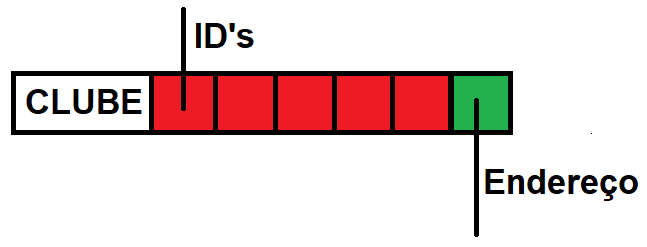
\includegraphics[width=.4\textwidth]{lista.png}
\caption{Estrutura da Lista Invertida}
\label{fig:create1}
\end{figure}

\subsubsection{Criar id na lista}
Para criar a lista seria necessário saber se a palavra se encontra na lista, para poder adicionar apenas o id, senão dese-se adicionar a somente o id na frente da palavra. Para estabelecer isso na frente de uma palavra seria possivel adicionar apenas 5 ids e a ultima posição estaria disponivel para o endereço da proxima posição da palavra onde iria armazenar mais arrays. Foi escolhida essa implementação por facilitar a questão de leitura do arquivo, pois era necessário saber quantos ids deveriam ser lidos para chegar a próxima palavra.

\subsubsection{Deletar id da lista}
Para deletar um id na lista o algoritmo utilizado foi ler a palavra e começar a comparar o id, se caso o read byte for igual ao id o programa deve ir para a posicao onde se encontra o id e sobrepor com um -1, pois na lista invertida todos os dados com -1 significa que eles aquela posição está disponível para ser usada. Com isso, o id é excluído do arquivo da lista invertida.

\subsubsection{Atualizar id na lista}
Para atualizar a lista invertida o algoritmo utilizado foi excluir todos os dados relacionado ao id que foi atualizado, depois criar ele novamente no arquivo da lista para manter a ordenalidade e por questões de reutilização de código.

\section{Arquivo de índices}
Para a criação do arquivo de índices foi levado em consideração os ids e o endereço do objeto no arquivo de dados principal, então a listagem no arquivo seguiu o seguinte parâmetro (id, endereço). Para assim facilitar a busca no arquivo de índices.

\begin{figure}[ht]
\centering
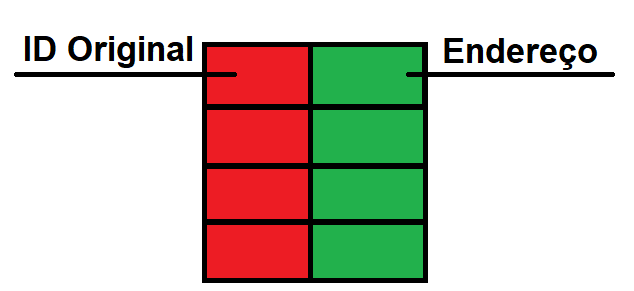
\includegraphics[width=.4\textwidth]{indice.png}
\caption{Estrutura do arquivo de índices}
\label{fig:create1}
\end{figure}

\subsection{Criar endereço do id no arquivo de índices}
Para criar o id no arquivo de índices foi levado em consideração o tamanho do arquivo, caso o arquivo tivesse tamanho 0 o objeto ia ser inserido na primeira posição, senão ele ia ser inserido na última posição do arquivo.

\subsection{Deletar id e endereço do arquivo de índices}
O metódo de deletar levou em consideração a busca por id, quando você queria deletar um objeto do arquivo, você passava o id desse objeto e fazia a busca do mesmo. Caso achasse o id você sobre escrevia o id e o edereço com o valor -1, como se fosse uma lápide dizendo que aquele local está inutilizável.

\subsection{Atualizar endereço no arquivo de índices}
O metódo de atualizar o arquivo de indices era utilizado caso o usuário fizesse alguma alteração em um clube que demandasse a mudança de localização dele do arquivo de dados original, com isso a implementação foi feita mandando o objeto do clube onde continha o id e o endereço novo do objeto, tendo isso o algoritmo fazia uma busca pelo id e quando o achava mudava o endereço que estava escrito no seu lado para o novo endereço no arquivo de dados original.
%%%%%%%%%%%%%%%%%%%%%%%%%%%%%%%%%%%%%%%%%%%%%%%%%%%%%%%%%%%%%%%%%%%%%%

\section{Testes e resultados do arquivo sequencial}
\subsection{Criação de um clube}
O primeiro passo para a criação do clube e escolher a opção. Após a seleção das informações seria necessário informar os dados para o programa, no exemplo forma criados dois times, com o intuito de mostrar a criação de partidas no próximo exemplo.

\newpage
\begin{figure}[ht]
\centering
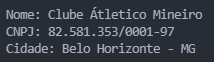
\includegraphics[width=.4\textwidth]{create_dados.png}
\caption{Criação clube 1}
\label{fig:create1}
\end{figure}

\begin{figure}[ht]
\centering
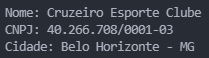
\includegraphics[width=.4\textwidth]{create_dados2.png}
\caption{Criação clube 2}
\label{fig:create2}
\end{figure}

Quando criados todos os dados são inseridos no arquivo, com isso pode-se observar que todos os dados foram inseridos com sucesso.

\begin{figure}[ht]
\centering
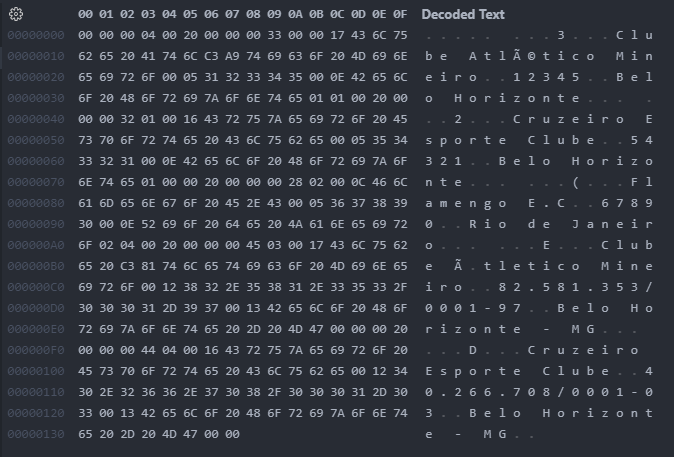
\includegraphics[width=.6\textwidth]{create_no_arquivo.png}
\caption{Dados criados inseridos no arquivo}
\label{fig:create_sucess}
\end{figure}

\subsection{Criação de partidas}
Para a criação de uma partida deve-se selecionar a opção desejada. Com isso, pode inserir os dados desejados para o programa, como mostrado e explicado nos CRUDs.

\newpage
\begin{figure}[h]
\centering
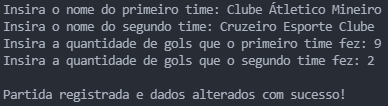
\includegraphics[width=.5\textwidth]{create_game_dados.png}
\caption{Inserção dos dados para o programa}
\label{fig:createGdados}
\end{figure}

Após todos os dados serem inseridos em terminal terá um update nos campos de pontos e partidas jogadas no arquivo para cada um dos times, como mostrado na Figura 6 do documento.

\begin{figure}[ht]
\centering
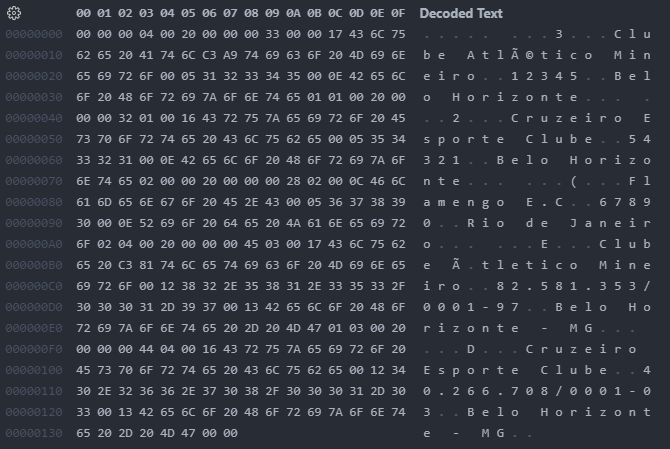
\includegraphics[width=.6\textwidth]{create_game_arquivo.png}
\caption{Resultado no arquivo após a inserção}
\label{fig:createGarquivo}
\end{figure}

\subsection{Procurar um time no arquivo}
Para procurar um time no arquivo, após selecionar a opção desejada basta apenas inserir o ID desejado que será mostrado todas as informações disponíveis para determinado clube.

\begin{figure}[ht]
\centering
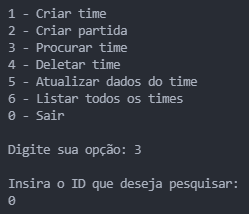
\includegraphics[width=.3\textwidth]{selection_option_and_id.png}
\caption{Seleção da opção desejava e passagem do ID}
\label{fig:readID}
\end{figure}

\newpage
\begin{figure}[ht]
\centering
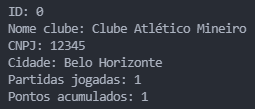
\includegraphics[width=.4\textwidth]{result.png}
\caption{Resultado da pesquisa por ID}
\label{fig:readID_result}
\end{figure}

\subsection{Atualizar dados do time}
Para o exemplo vamos mudar o nome de Cruzeiro Esporte Clube para Flamengo, além disso mudar o CNPJ e a cidade do clube.

\begin{figure}[ht]
\centering
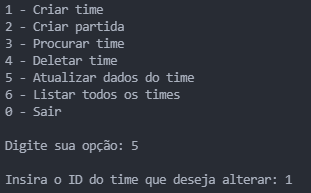
\includegraphics[width=.4\textwidth]{att_option.png}
\caption{Seleção e passagem do ID}
\label{fig:att_option}
\end{figure}

\begin{figure}[ht]
\centering
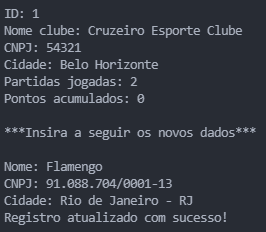
\includegraphics[width=.3\textwidth]{att_sucess.png}
\caption{Novos dados inseridos}
\label{fig:att_sucess}
\end{figure}

Quando fazemos a atualização pode-se ver que dependendo da quantidade de bytes a serem inseridos pode ser modificado de formas diferentes como mostrado na seção CRUD - Update. Com isso, o resultado do arquivo após a atualização está sendo mostrado na Figura 11 do documento.

\newpage
\begin{figure}[ht]
\centering
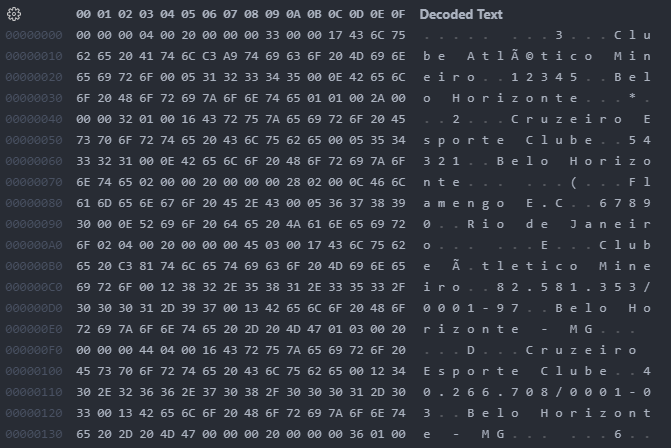
\includegraphics[width=.6\textwidth]{att_arquivo.png}
\caption{Resultado no arquivo}
\label{fig:att_arq}
\end{figure}

\subsection{Deletar clube}
Ao deletar um clube uma lápide é inserida no arquivo.

\begin{figure}[ht]
\centering
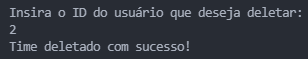
\includegraphics[width=.7\textwidth]{delete.png}
\caption{Passagem dados}
\label{fig:att_arq}
\end{figure}

\begin{figure}[ht]
\centering
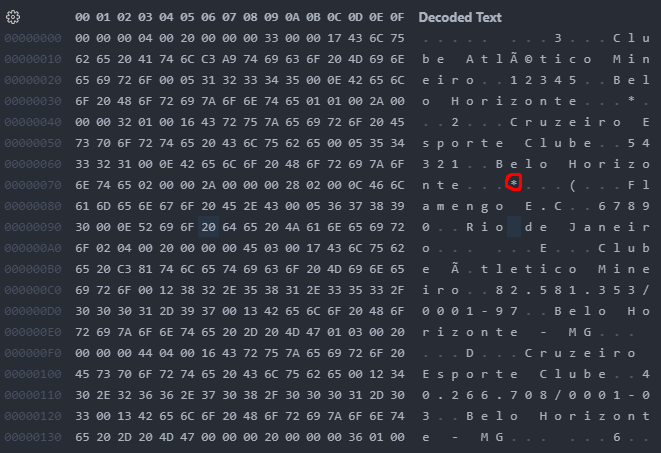
\includegraphics[width=.5\textwidth]{delete_result.png}
\caption{Resultado no arquivo após deletar clube}
\label{fig:att_arq}
\end{figure}

\subsection{Buscar ID's na lista invertida}
Para o teste vamos criar 4 times: Clube Atlético Mineiro (ID = 0, Belo Horizonte), Clube Regatas do Flamengo (ID = 1, Rio de Janeiro), Cruzeiro Esporte Clube (ID = 2, Belo Horizonte) e Vasco da Gama (ID = 3, Rio de Janeiro). E para testar o algoritmo de busca na lista invertida vamos fazer duas buscar por nome e duas buscas por cidade, utilizando as seguintes informações Clube e Rio, respectivamente.

\newpage
\subsubsection{Busca feita por nome}

\begin{figure}[ht]
\centering
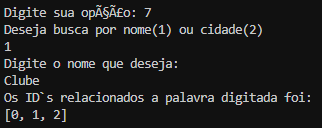
\includegraphics[width=.6\textwidth]{busca_nome.png}
\caption{Resultado da busca feita por nome na lista invertida}
\label{fig:att_arq}
\end{figure}

\subsubsection{Busca feita por cidade}

\begin{figure}[ht]
\centering
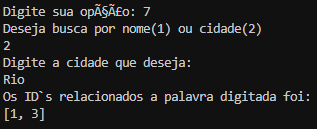
\includegraphics[width=.6\textwidth]{busca_cidade.png}
\caption{Resultado da busca feita por cidade na lista invertida}
\label{fig:att_arq}
\end{figure}

\subsection{Arquivo de índices}
O teste no arquivo de índices foi feito a partir de uma função especifica não disponível para o usuário, apenas para o programador testar. Então para o teste foi efetuado a criação de 4 times (os mesmos criados no buscar id's na lista invertida e foram deletados, atualizados para ver se a alteração acontecia no arquivo de índices.

\begin{figure}[ht]
\centering
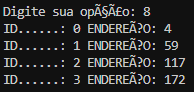
\includegraphics[width=.4\textwidth]{arquivo_antes_delete.png}
\caption{Arquivo de índices antes da modificação}
\label{fig:att_arq}
\end{figure}

\newpage
\subsubsection{Deletar no arquivo de índices}
Após deletar o id e endereço do arquivo o resultado esperado e não mostrar mais para o programador quando \textit{printar} o arquivo inteiro.

\begin{figure}[ht]
\centering
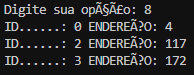
\includegraphics[width=.4\textwidth]{arquivo_depois_delete.png}
\caption{Arquivo de índices depois do delete}
\label{fig:att_arq}
\end{figure}

\subsubsection{Atualizar no arquivo de índices}
Após atualizar o id e endereço do arquivo o resultado esperado e mostrar para o programador a nova posição do id atualizado.

\begin{figure}[ht]
\centering
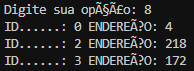
\includegraphics[width=.4\textwidth]{apos_update.png}
\caption{Arquivo de índices depois de atualizar o ID 2}
\label{fig:att_arq}
\end{figure}


\section{Ordenação externa}
Infelizmente o grupo não conseguiu implementar de forma correta a ordenação externa. Para não prejudicar o restante do trabalho optamos por armazenar todos os id's no arquivo de índices já de forma ordenada, para possibilitar a implementação de outros requisitos impostos no trabalho.
%%%%%%%%%%%%%%%%%%%%%%%%%%%%%%%%%%%%%%%%%%%%%%%%%%%%%%%%%%%%%%%%%%%%%%
\section{Conclusão}
De acordo com o resultado dos testes, percebemos que o programa está funcionando  de forma correta, conseguindo cobrir todos os tipos de situações que podem ser causadas por dados inseridos pelo usuário sendo eles válidos ou não. Além disso pode-se observar a grande importância da utilização do arquivo de índices juntamente da substituição da busca sequencial por uma busca binária no arquivo de índices que estava ordenado utilizando uma ordenação na inserção dos id's, melhorando assim a performance da busca. O programa também utilizou uma lista invertida para facilitar a busca do usuário quando era necessário busca os id's relacionados a determinada palavra (nome e/ou cidade). Pode-se observar então que o programa está em pleno funcionamento com muitas opções para facilitar a interação do usuário.


\end{document}
